\documentclass[NET,english,beameralt]{tumcd/tumbeamer}

% If you load additional packages, do so in packages.sty as figures are build
% as standalone documents and you may want to have effect on them, too.

% Configure author, title, etc. here:

% End video

% Header
% \newcommand{\zwischentitel}{Seminar Presentation}
% \newcommand{\leitthema}{Title}
% End Header

% Titlepage
% \title{The Eternal Adversary between Censor and
% Circumvention}
% \author{Guanru Chen}
% \newcommand{\presdatum}{December 2024}
% \institute
% {
%   Technische Universität München\\
% }
% \subtitle{ Technical Perspective}
% End Titlepage


% Slides
% \begin{document}

% 1. Slide: Titlepage
% \begin{frame}
% 	\titlepage
% \end{frame}

% 2. Slide: TOC
\begin{frame}
   \frametitle{Contents and sections of presentation}
   \tableofcontents[subsectionstyle=hide]
\end{frame} 

% Further Slides
% \section{Titles} 
% \begin{frame}
%    \frametitle{Title} 
%    Each frame should have a title.
% \end{frame}

\section{Prologue}
\begin{frame}
    % \frametitle{Prologue}
    \begin{quote}
        ``Life is dear, love is dearer. Both can be given up for freedom.`` \\
        --- Sandor Petöfi
    \end{quote}
    
\end{frame}

\section{Methods}
\subsection{Data Collection}
\begin{frame}
Some common ways to collect network traffic in different OSI layers
\small
\begin{itemize}
    \item HTTP(s) Proxies like Charles Proxy, fiddler, and Proxyman, are widely used in web debugging. When you open the developer tool in your browser, you are actually analyzing network traffic. 
    \item Packet capture tools that integrated with systems' network stack. The most famous and classic example is TCPDump and Wireshark.
    There is a new remarkable approach in the Linux platform called eBPF (extended Berkeley Packet Filter), which is the successor of the classic BPF (Berkeley Packet Filter). It is an interesting and popular topic that is worth further investigation. For portability reasons, in our research, we still use the classical one. 
    \item Physical layer collection needs more special equipment, such as optical splitters and optical fiber detectors, that makes it possible to capture modulated physical signals. It is not so common, but it can still be utilized by national agencies.
\end{itemize}

\end{frame}

% \begin{frame}\frametitle{Lists with Pause}
%    \begin{itemize}
%       \item Introduction to  \LaTeX \pause 
%       \item Second bullet point \pause 
%       \item And a third one \pause 
%       \item The last one
%    \end{itemize} 
% \end{frame}

% \begin{frame}{Use TCPDump Tool}
% \begin{lstlisting}[language=bash]
%     tcpdump -G <capture interval> -W 1 -w <protocol name>.pcap -i <network interface> -n dst host <ip> and dst port <port> and <transmission protocol> --print
% \end{lstlisting}
% Specifying the enclosed parameters accordingly provides flexibility to filter traffic and interact with it.
% \end{frame}

\subsection{Use TCPDump \cite{tcpdump} Tool}
\begin{frame}[fragile]
% \frametitle{Use TCPDump \cite{tcpdump} Tool}
    TCPDump can capture, filter, and store designated traffic with given parameters. For more detail, please refer to its \href{https://www.tcpdump.org/}{manual}
   \lstset{language=bash, basicstyle=\small \ttfamily, showspaces=false,   showtabs=false, tab= , keywordstyle=\bfseries,     showstringspaces=false, framexleftmargin=5mm, frame=single,     numbers=left,
    numberstyle=\tiny,
    stepnumber=1,
    numbersep=5pt,
    texcl=true, 
    breaklines=true,
    breakatwhitespace=true,
    keepspaces=true,
    columns=fullflexible,}
    \begin{lstlisting}
    tcpdump -G <capture interval> -W 1 -w <protocol name>.pcap -i <network interface> -n dst host <ip> and dst port <port> and <transmission protocol> --print
    \end{lstlisting}
    Specifying the enclosed parameters accordingly provides flexibility to filter traffic and interact with it.
    It is possible to automate the process in order to collect larger-scale datasets.
\end{frame}


\subsection{Data Analysis and Plot}
\begin{frame}
% \frametitle{Data Analysis and Plot}

\small
Regarding passive (static) traffic analysis, we consider these factors: packet length, entropy, TLS fingerprint (if it has one), and those factors in the temporal domain.
We should retrieve encrypted TCP payload from captured Ethernet frames first. 
For analysis, we use library dpkt \cite{dpkt} and for visualization we use \href{https://matplotlib.org/}{matplotlib}

\begin{figure}
    \centering
    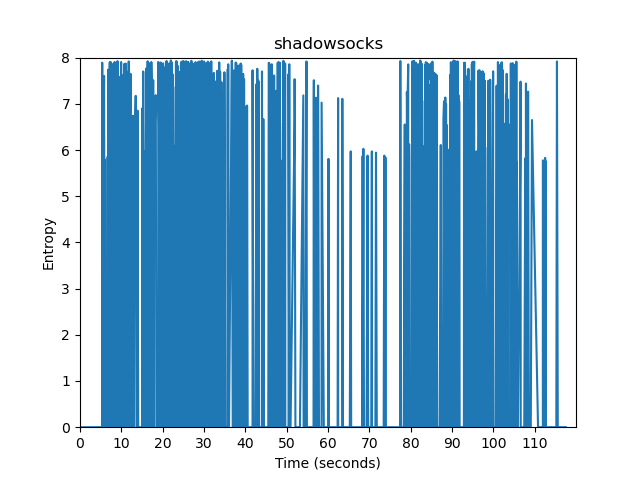
\includegraphics[scale=0.35]{pics/plot.png}
    \caption{\tiny A sample plot of Shadowsocks protocol.}
    \label{fig:enter-label}
\end{figure}
    
\end{frame}

\subsection{Server Configuration}
\begin{frame}
    % \frametitle{Server Configuration}

    A few configurations may be needed to set up a proxy server.

    \begin{itemize}
    \item Install the server-side software, use package manager if possible.
    \item Basic configuration. It will be required for almost all proxy protocols, in which you provide basic information, e.g. address, port to listen, and credentials for authorization.  
    \item Obtain a SSL certificate if TLS should be used and maintain it e.g. renew it timely and adapt security response.
    \item Set up a fallback server (more details of fallback we will discuss later in section \ref{sec:fallback}).
    \end{itemize}
\end{frame}

\subsection{Protocols}
\begin{frame}
    % \frametitle{Protocols to Research}
    We choose some typical protocols according to their features.
    \begin{table}[h]
    \begin{tabular}{|c|c|c|c|}
      \hline
      \diagbox{Protocol}{Feature} & TLS & Packet Length Padding & Fallback \\ \hline
      Shadowsocks\cite{Shadowsocks} & \texttimes & \checkmark & \texttimes \\ \hline
      Obfs4\cite{Obfs4} & \texttimes & \checkmark & \texttimes \\ \hline
      Trojan\cite{Trojan_gfw} & \checkmark & \texttimes & \checkmark \\ \hline
      Naiveproxy\cite{Naiveproxy} & \checkmark & \checkmark & \checkmark \\ \hline
    \end{tabular}
    \end{table}
\end{frame}

\subsection{Technical Details}
\subsection{Fallback}\label{sec:fallback}
\begin{frame}
    % \frametitle{Fallback}
    \begin{figure}
        \centering
        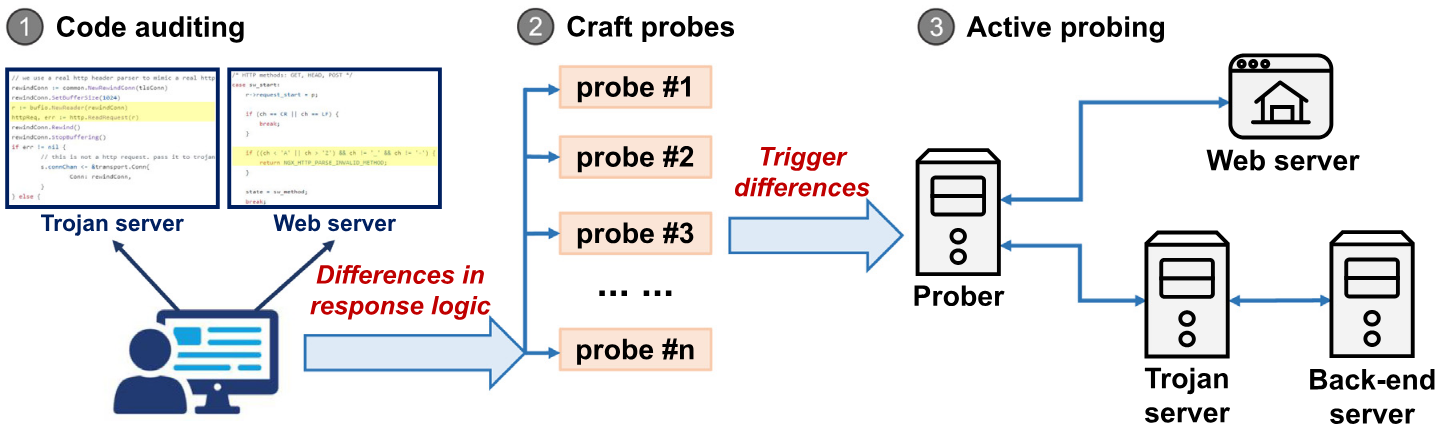
\includegraphics[scale=0.20]{pics/fallback.png}
        \caption{How fallback works in combat of probe \cite{Trojan-Probe}}
        \label{fig:fallback}
    \end{figure}
\end{frame}

\subsection{Supportive resources}
\begin{frame}
% \frametitle{Supportive Resources}
    We publish related files in \href{https://gitlab.lrz.de/tuinh09/teaching/scni/repos/2024ws-hn/u157}{the project's repository}
    \begin{itemize}
        \item Configuration snippets can be found under folder \texttt{resources/Config}. "$<>$" enclosed values should be replaced accordingly.
        \item Manuals and notes are under folder \texttt{resources/Manual}.
    \end{itemize}
    
\end{frame}

\section{Topics}
\subsection{Entropy}
\begin{frame}
    % \frametitle{Entropy}
    The entropy can be calculated as $H = -\sum_{i=1}^{n} p_i \log_2(p_i)$. It represents how disordered a message is. Highly encrypted messages are near to random data.
    It is also practical to consider the variation of entropy in the clock domain.
    \begin{table}[h]
    \centering
    \caption{Average entropy for common protocols}
    \resizebox{\columnwidth}{!}{
        \begin{tabular}{|l|lllll|}
        \hline
        \multirow{2}{*}{} & \multicolumn{5}{c|}{Protocol Name}                                                                                                   \\ \cline{2-6} 
                          & \multicolumn{1}{l|}{Shadowsocks} & \multicolumn{1}{l|}{HTTPS} & \multicolumn{1}{l|}{NaiveProxy} & \multicolumn{1}{l|}{Trojan} & Obfs4 \\ \hline
        Entropy          & \multicolumn{1}{l|}{7.999}      & \multicolumn{1}{l|}{7.977} & \multicolumn{1}{l|}{7.992}      & \multicolumn{1}{l|}{7.858}  & 7.999 \\ \hline
        \end{tabular}%
    }
    \end{table}
\end{frame}

\subsection{Packet Length}
\begin{frame}
    % \frametitle{Packet Length}
    
    % \small
    Packet length is a significant factor in a protocol. Specifically, we should only consider its payload (i.e. Server Data Unit).
    When using statistical methods to inspect it, an outlier can be remarkable. For example, as is shown in the paper, the Trojan protocol does not adopt a long packet resizing mechanism.
\begin{figure}[H]
    \centering
        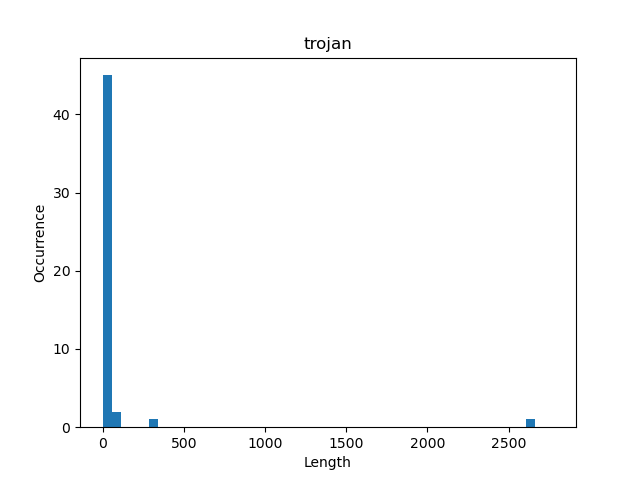
\includegraphics[scale=0.45]{pics/occurrence_of_length_trojan.png}
    \caption{Length-occurrence statistics}
\end{figure}
\end{frame}

\subsection{TLS Fingerprinting}
\begin{frame}
    % \frametitle{TLS Fingerprinting}
    
    \small
    As the SSL/TLS handshake happens in most plain text, the features of such a connection can be identified. For example, \texttt{TLS\_ECDHE\_RSA\_WITH\_CHACHA20\_POLY1305\_SHA256} shows cipher suites, both symmetric and asymmetric, hash function, and key exchange algorithm; they are typical TLS fingerprints. Besides, there are further features such as SSL versions and certificates. 
    All these factors composite a vector that can be categorized by algorithms (machine learning is needed).
    \begin{figure}
        \centering
        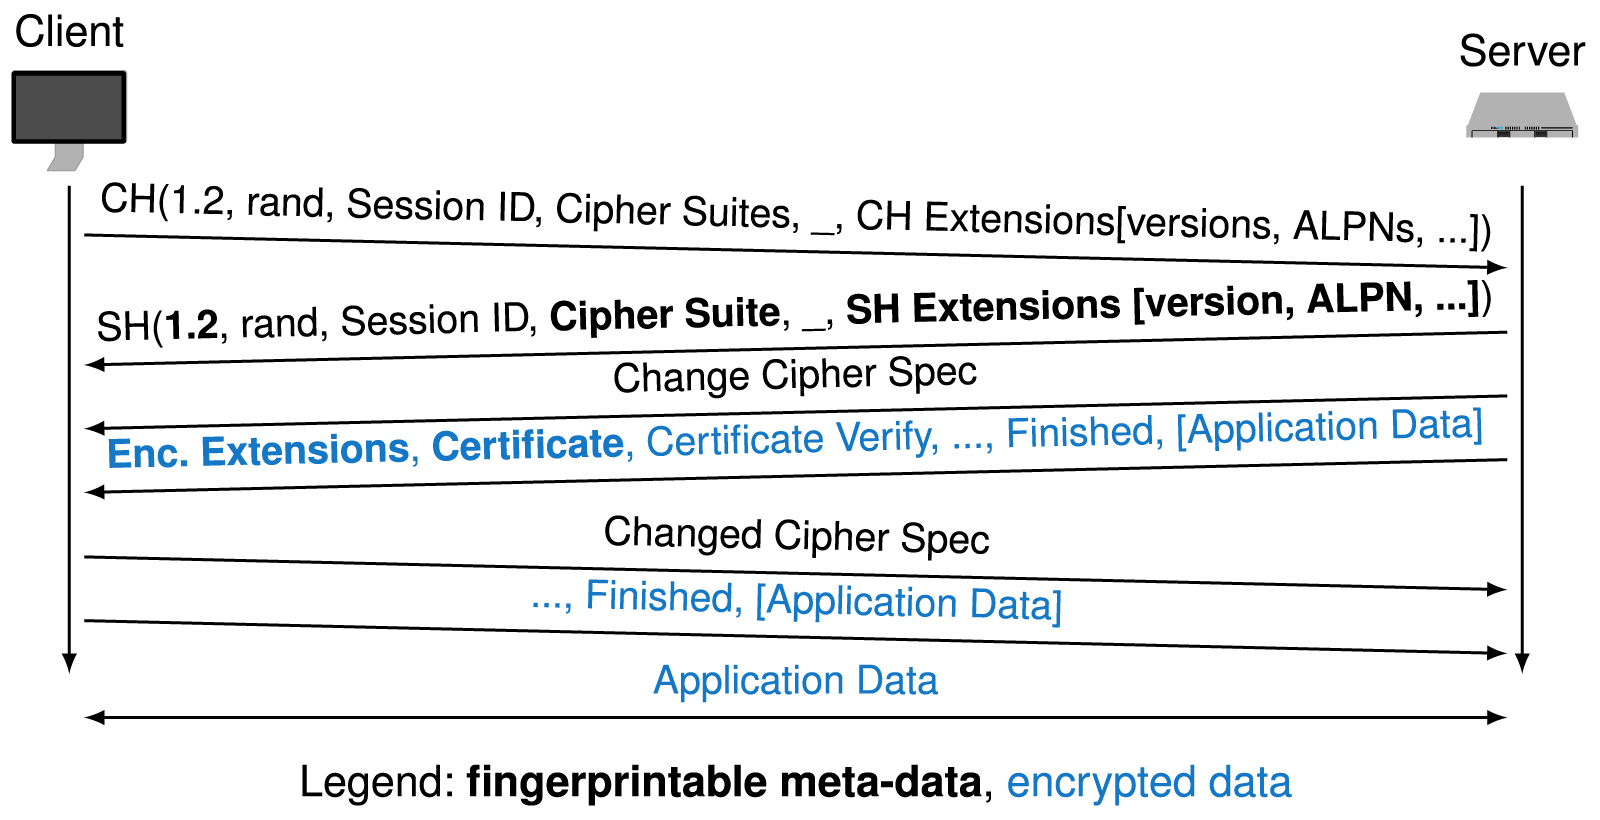
\includegraphics[scale=0.15]{pics/TLS_Handshake.png}
        \caption{\small TLS handshaking \cite{TLS_handshake}}
        \label{fig:fallback}
    \end{figure}
\end{frame}

\subsection{SNI/CH technologies}
\begin{frame}
    % \frametitle{SNI/CH Technologies}

    In SSL/TLS handshaking processes, there is a remarkable phase, client hello (CH), that provides more information for the server along with TCP/IP 5 tuple and domain name, which will be especially useful when CDN or reverse proxy is enabled.
    But it is firstly designed without taking privacy into consideration, so the primeval version of CH is in plain text, which exhibits information about the connection and makes the SNI-based block possible.
    It has successors that try to mitigate the privacy defect, called eSNI and ECH, whose e stands for encrypted, but they are not widely adopted yet.
    \begin{figure}
        \centering
        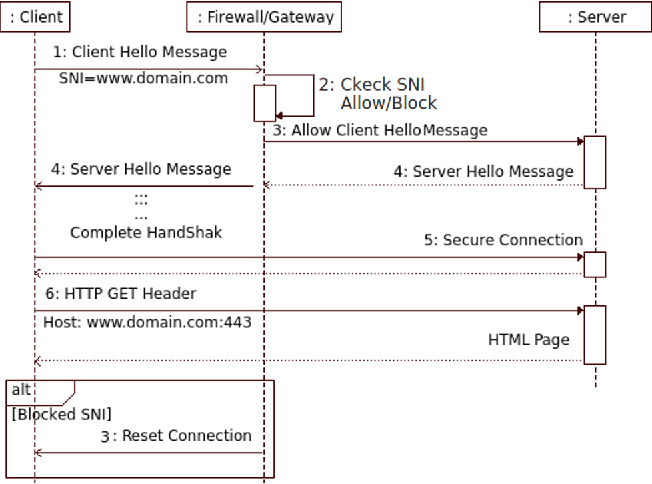
\includegraphics[scale=0.25]{pics/SNI_Block.png}
        \caption{\small SNI based block \cite{SNI_block}}
        \label{fig:fallback}
    \end{figure}
\end{frame}


% \section{Colors}
% \begin{frame}
%    \frametitle{An Overview of TUM's Colors}
%    \tiny{Color blue sRGB 100\%: 0-101-189} \\
%    \colorbox{tumcolor-blue}{}{}  \\
%    \vspace{0.5cm}
%    \tiny{Color green sRGB 100\%: 162-173-0} \\
%    \colorbox{tumcolor-green}{}{} \\
%    \vspace{0.5cm}
%    \tiny{Color light grey sRGB 100\%: 218-215-203} \\
%    \colorbox{tumcolor-lightgrey}{}{} \\
%    \vspace{0.5cm}
%    \tiny{Color orange sRGB 100\%: 227-114-34} \\
%    \colorbox{tumcolor-orange}{}{} \\
%    \vspace{0.5cm}
% \end{frame}

\section{Conclusion}
\begin{frame}
    % \frametitle{Conclusion}
    In conclusion, the central of network censorship circumvention is camouflage or \textbf{collateral freedom}. In practice, both efforts are based on the nature of OSI layers.
    We can neither cover all the topics nor dive deep into all subdomains. This project gives an overview of these technologies.
\end{frame}

\section{Afterword}
\begin{frame}
    % \frametitle{Afterword}
    \small
    After finishing this project, I thought a lot and put some of my thoughts in the afterword out of my selfishness.
    All technologies will not stay in academia but will finally enter the real world and be entangled with "impure" factors like ethics, society, and the environment.
    
    So I believe that as technicians (or technicians in the future), we should have a sense of social responsibility and ethics, especially when we are dealing with technology. And that is what I demand myself.

    After all, I hope that everyone can recognize and understand Freedom of speech (including but not limited to Internet freedom) is all the citizens' right, that can never be deprived.

   \begin{figure}
      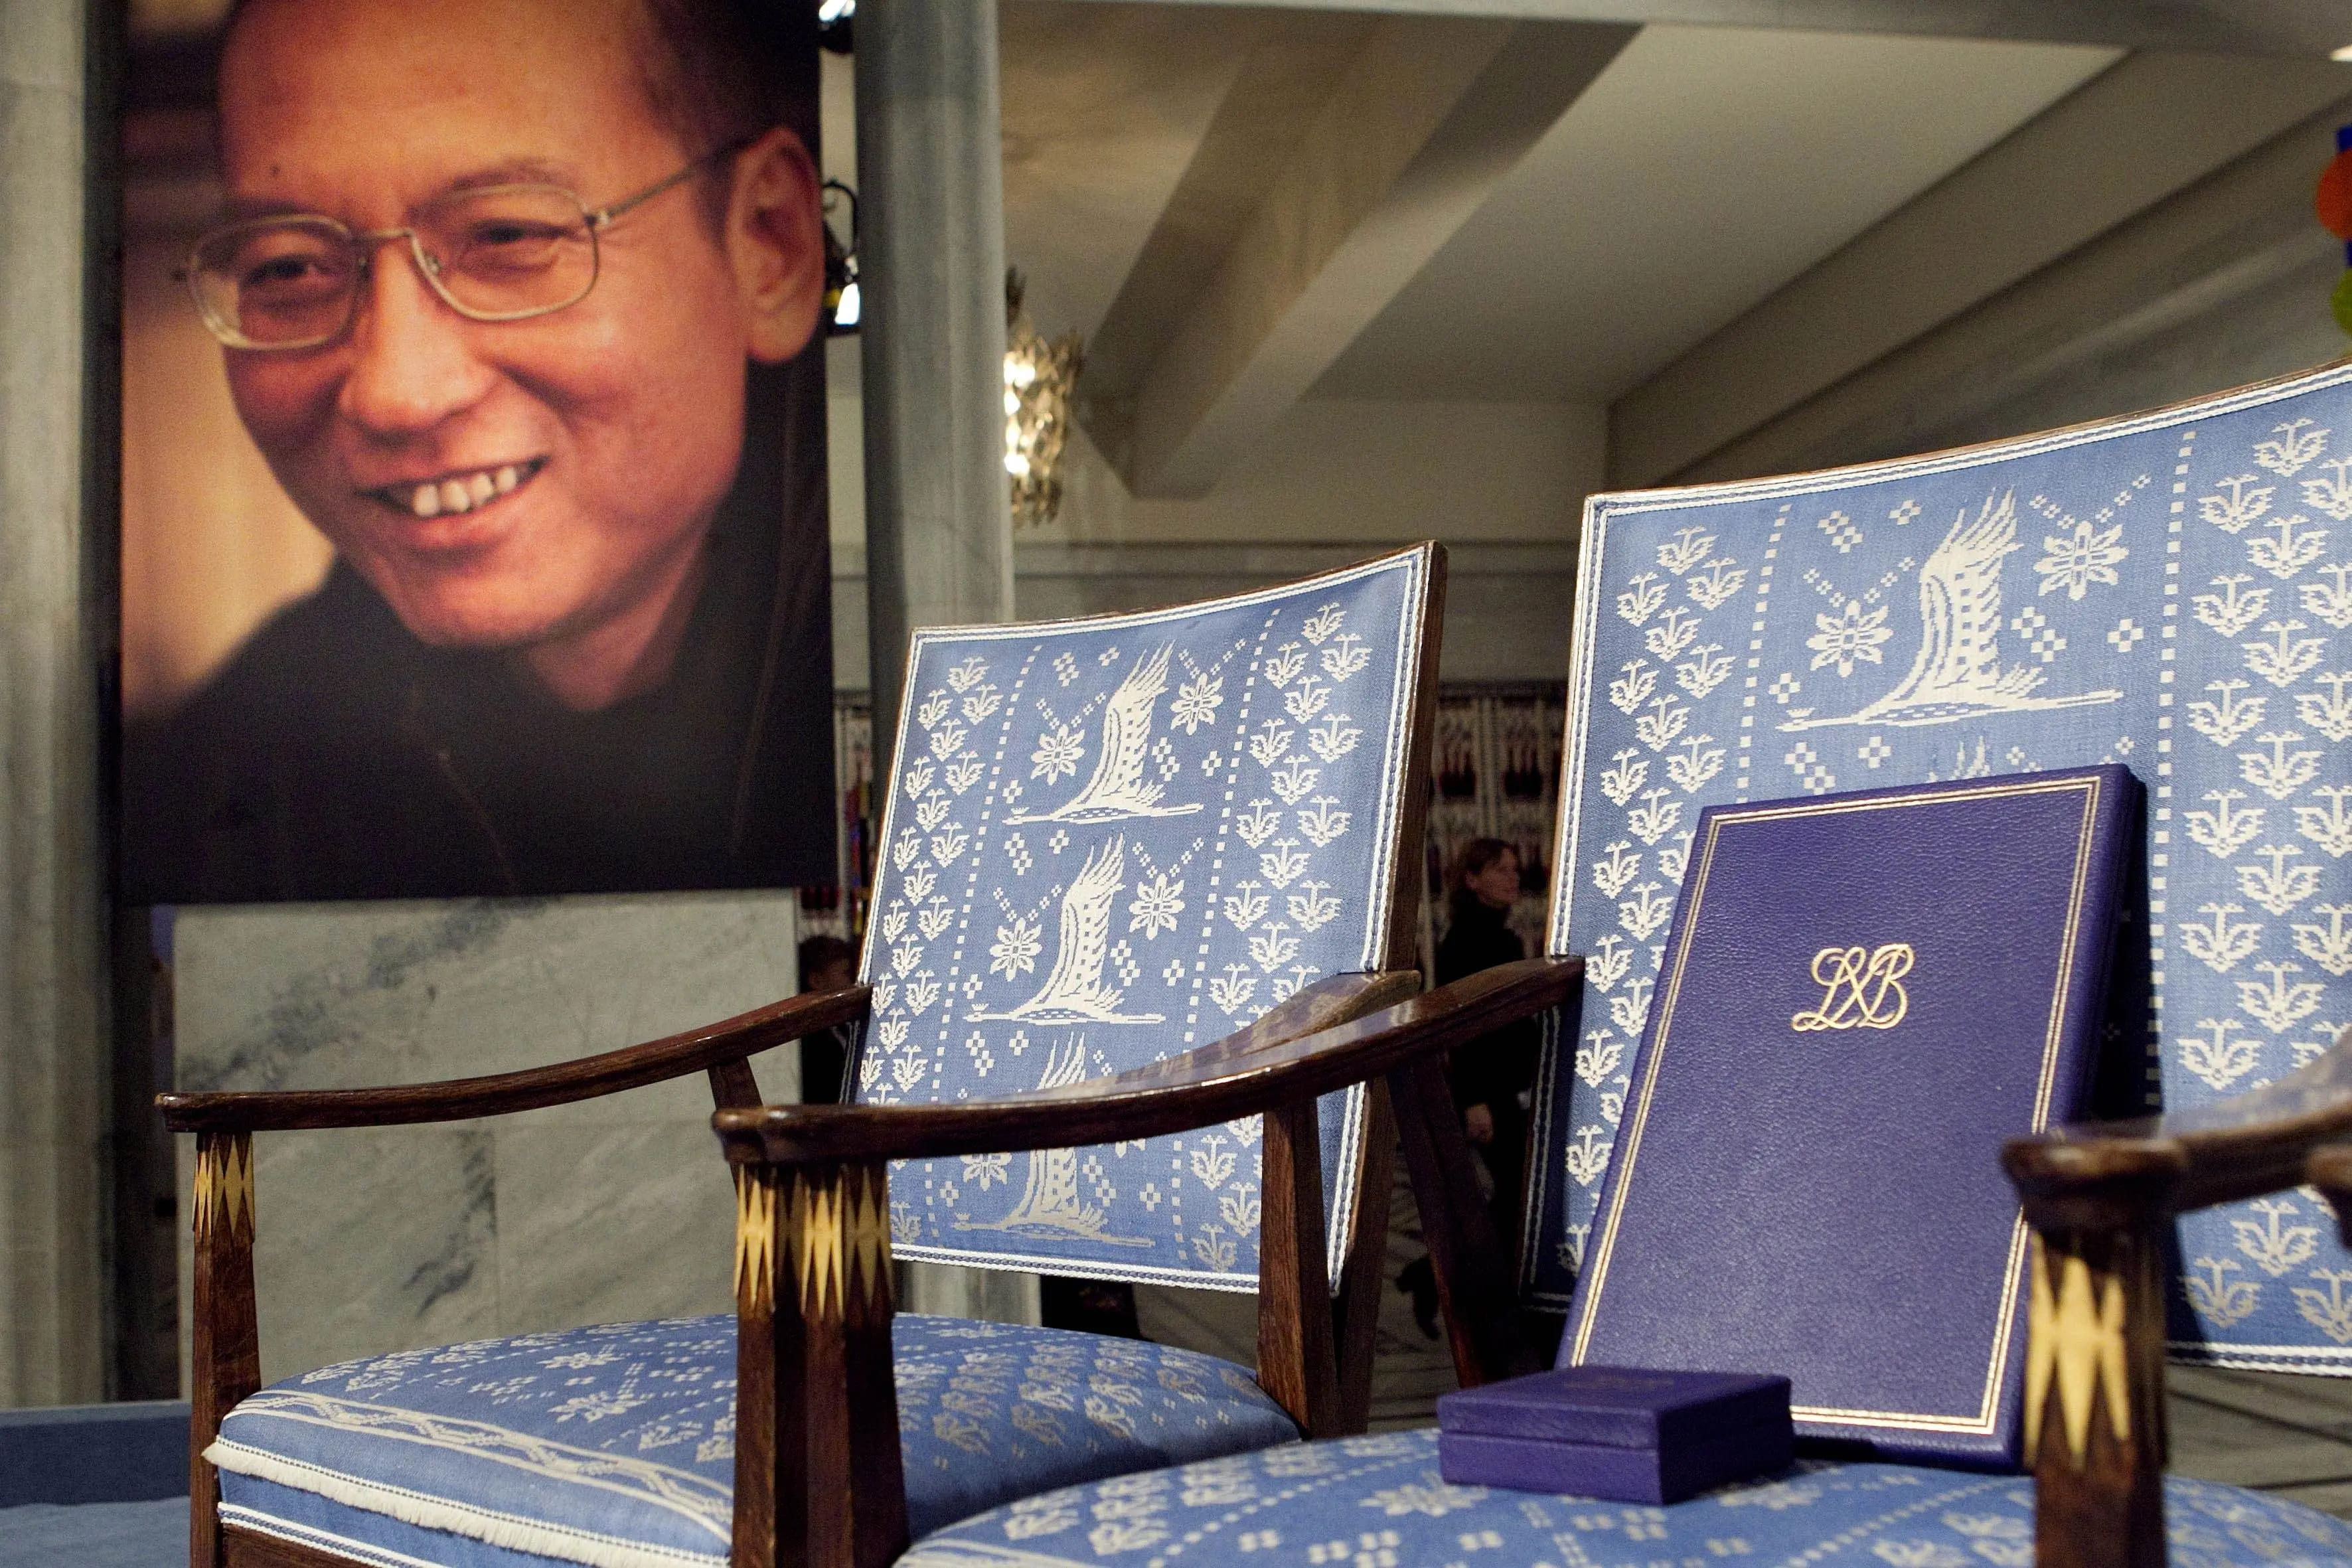
\includegraphics[scale=0.05]{pics/XiaoboLiu_Nobel} 
      \caption{Dr. Xiaobo Liu, Nobel Peace Prize winner of 2010\cite{Dr_xiaobo_liu}}
   \end{figure}

\end{frame}



% \subsection{Code Listings} 
% % The [fragile] is important for listings!
% \begin{frame}[fragile]
%    \frametitle{Don't Ever Bore the Audience with Code Listings}
%    \lstset{language=C, basicstyle=\small \ttfamily, showspaces=false, showtabs=false, tab= , keywordstyle=\bfseries, showstringspaces=false, framexleftmargin=5mm, frame=single, numbers=left, numberstyle=\tiny, stepnumber=1, numbersep=5pt, texcl=true}
%    \begin{lstlisting}[caption={Especially when they are erroneous},frame=tlrb]
% #include <stdio.h>

% int main(void)
% {
%   printf("Hallo Welt\n");
%   while(1);
%   return 0;
% }
%    \end{lstlisting}
% \end{frame}

% \begin{frame}[allowframebreaks]
% \frametitle{Bibliography}
%     \printbibliography
% \end{frame}

% \end{document}


\begin{document}

% If you are preparing a talk but do not like the default font sizes, you may
% want to try the class option 'beameralt', which uses smaller default font
% sizes and integrates subsection/subsubsection names into the headline.

% For lecture mode, you may want to build one set of slides per chapter but
% with common page numbering. If so,
% 1) create a new .tex file for each chapter, e.g. slides_chapN.tex,
% 2) set the part counter to N-1 (assuming chapters start at 0), and
% 3) and name your chapter by using the \part{} command.
%\setcounter{part}{-1}
%\part{Organisatorisches und Einleitung}

% For 16:9 slides, use the class option 'aspectratio=169'.

% If class option 'noframenumbers' is given, frame numbers are not printed.

% If class option 'notitleframe' is given, the title frame is not autmatically
% generated.

% Class option 'nocontentframes' suppresses automatic generation of content
% frames when new parts/sections are started.

% Include source files from ./include (or ./include/chapN).
\documentclass{standalone}
\usepackage{tumcolor}
\usepackage{tikz}
\usepackage{pgfplots}
\pgfplotsset{compat=newest}
\usepgfplotslibrary{units}

\usepackage[binary-units]{siunitx}
\DeclareSIUnit[per-mode=symbol]\bps{\bit \per \second}
\DeclareSIUnit[per-mode=symbol]\kbps{\kilo\bps}
\DeclareSIUnit[per-mode=symbol]\Mbps{\mega\bps}
\DeclareSIUnit[per-mode=symbol]\Gbps{\giga\bps}
\sisetup{detect-all}

\begin{document}
\begin{tikzpicture}

% Read data from CSV file
\pgfplotstableread[col sep = semicolon]{data/testdata.csv}\data

\begin{axis}[
	width=10cm,
	height=5cm,
	xmin = 0, xmax = 10,
	ymin = 0, ymax = 10,
	xlabel={Time},
	ylabel={Rate},
	x unit = \si{\milli \second},
	y unit = \si{\Mbps},
	scaled ticks=false,
	tick label style={/pgf/number format/fixed},
	no marks,
	grid=both,
	legend pos = south east,
]
	\addplot[TUMRed, domain=0:10, samples=500] {0.04* (x-5)^3 + 5};
	\addplot[TUMBlue, only marks] table[x index = {0}, y index = {1}]{\data};

	\legend{Estimation, Samples}
\end{axis}

\end{tikzpicture}
\end{document}


% Include markdown source from ./pandoc
%\documentclass{standalone}
\usepackage{tumcolor}
\usepackage{tikz}
\usepackage{pgfplots}
\pgfplotsset{compat=newest}
\usepgfplotslibrary{units}

\usepackage[binary-units]{siunitx}
\DeclareSIUnit[per-mode=symbol]\bps{\bit \per \second}
\DeclareSIUnit[per-mode=symbol]\kbps{\kilo\bps}
\DeclareSIUnit[per-mode=symbol]\Mbps{\mega\bps}
\DeclareSIUnit[per-mode=symbol]\Gbps{\giga\bps}
\sisetup{detect-all}

\begin{document}
\begin{tikzpicture}

% Read data from CSV file
\pgfplotstableread[col sep = semicolon]{data/testdata.csv}\data

\begin{axis}[
	width=10cm,
	height=5cm,
	xmin = 0, xmax = 10,
	ymin = 0, ymax = 10,
	xlabel={Time},
	ylabel={Rate},
	x unit = \si{\milli \second},
	y unit = \si{\Mbps},
	scaled ticks=false,
	tick label style={/pgf/number format/fixed},
	no marks,
	grid=both,
	legend pos = south east,
]
	\addplot[TUMRed, domain=0:10, samples=500] {0.04* (x-5)^3 + 5};
	\addplot[TUMBlue, only marks] table[x index = {0}, y index = {1}]{\data};

	\legend{Estimation, Samples}
\end{axis}

\end{tikzpicture}
\end{document}


% Comment out if you do not want a bibliography
\section{Bibliography}
\begin{frame}[allowframebreaks]
    \bibliographystyle{abbrv}
    \setbeamertemplate{bibliography item}[text]
    \footnotesize
    \bibliography{lit}
\end{frame}

\end{document}

